\chapter[Detección de hidrocarburos en aguas del RdP]{Detección y cuantificación de derrames de hidrocarburos en aguas ópticamente complejas del Río de la Plata utilizando sensores ópticos.}
\label{oil}

Previo al advenimiento de la tecnología satelital, la detección y caracterización de derrames de hidrocarburos sobre cuerpos de agua se realizaba visualmente desde aeronaves. En la actualidad, si bien la inspección visual sigue siendo la primera herramienta frente a dichas emergencias, la detección y caracterización ha evolucionado drásticamente gracias a la ayuda de los sensores remotos ópticos. Dichos sensores facilitan ampliamente la realización de diagnósticos tempranos - imprescindibles ante el surgimiento de un evento de derrame - permitiendo caracterizar el área afectada, la cantidad derramada, la dirección a la cual se dirige el derrame, entre otras cosas.
%
Si bien existen antecedentes sobre diferentes metodologías de detección no supervisadas de derrames en cuerpos de agua, todas están enfocadas en la detección en aguas ópticamente claras, donde muchas veces los derrames pueden ser confundidos con otros fenómenos naturales como ondas de gravedad internas, algas, compuestos orgánicos naturales, floraciones fitoplanctónicas, sombras de nubes, entre otros.
%
Considerando: la falta de investigación sobre las características espectrales dada por la presencia de hidrocarburos sobre aguas turbias; el derrame histórico ocurrido sobre el RdP frente al Partido de Magdalena (Prov. de Buenos Aires) en enero de 1999; la alta probabilidad de que vuelva a ocurrir un incidente de características similares dado el intenso tráfico marino, y en vistas a explotar las misiones satelitales argentina SAOCOM y SABIA-MAR, nos propusimos, en el presente capítulo, caracterizar experimentalmente la reflectancia espectral de una emulsión de hidrocarburos con aguas turbias con el fin de extraer potenciales índices espectrales que permitan distinguir las diferentes características de una muestra de agua turbia del RdP a diferentes espesores de hidrocarburos.
%
Para ello armamos una muestra de aguas del RdP a escala de laboratorio a la cual fuimos vertiendo diferentes volúmenes de hidrocarburos, y habiendo expuesto dicha muestra a condiciones de iluminación natural, medimos las reflectancias del agua a diferentes espesores de hidrocarburos. Los resultados nos muestran que existen varios índices espectrales que podrían auspiciar de indicadores de presencia de hidrocarburos en aguas turbias, como el cociente de reflectancias roja e infrarroja, la luminosidad, la turbidez o el cociente violeta/rojo. Si bien las diferencias halladas entre las firmas de aguas con hidrocarburos y aguas del RdP a diferentes espesores de hidrocarburos son contundentes, es fundamental ampliar este estudio para contemplar el impacto de otras variables pertinentes, como el SPM, diferentes tipos de hidrocarburos, diferentes grados de emulsión, etc.

$\quad$

\noindent
Los contenidos del presente capítulo se hallan desarrollados en el siguiente informe técnico:

$\quad$

\noindent
GOSSN, JUAN I.; GRINGS, F.M.; ROITBERG, E.; MORANDEIRA, N.; DOGLIOTTI, A.I.; FRANCO, M.; BARBER, M.; SALVIA, M. (2018) Caracterización de derrames utilizando técnicas de polarimetría SAR. Informe de avance del Proyecto AO para el desarrollo de Aplicaciones en el Área Oceanográfica con Imágenes SAR de la Misión SAOCOM CONICET(IAFE)/CONAE (2016-2018). Entregables 3 - 2018-12-04; p.1 - 21, \cite{gossn2018a}

\section{Introducción}
\label{oil:s:intro}

    Es bien sabido que los derrames de petróleo en cuerpos de agua afectan al medio ambiente, la economía y la calidad de vida de los habitantes costeros, siendo por ej. de público conocimiento que la fauna marina y costera expuesta al petróleo sufre tanto problemas de salud inmediatos como cambios a largo plazo en su fisiología y comportamiento, \cite{alonso2007}\cite{bendavid2000}\cite{ridoux2004}.
    %
    Es por estos motivos que para los países con una gran extensión costera es esencial la planificación de contingencia ante derrames. Esto es particularmente importante para la Argentina, donde muchos de los derrames ocurridos históricamente acontecieron en zonas costeras donde es mayor la densidad de rutas marítimas. De hecho, el derrame más caudaloso del que hay registro en el litoral argentino ocurrió en el RdP frente a la ribera del partido de Magdalena al noreste de la Provincia de Buenos Aires, donde se registró el derrame de 5500 $m^{3}$ de crudo \textit{Hydra} de origen submarino tras el impacto del buque \textit{Estrella Pampeana} (de la empresa Shell) con el buque \textit{Sea Paraná} de bandera alemana, Domínguez et al. 2009, \cite{dominguez2009}.
    %
    Dada entonces la mayor probabilidad de registrar derrames en aguas en zonas costeras como El Rincón en Bahía Blanca o el RdP - es decir, aguas turbias - es de particular interés poder identificar características espectrales distintivas de los derrames producidos sobre este tipo de aguas que sean detectables remótamente por sensores ópticos de color del mar. En particular,  en aguas claras, ya existen algoritmos cuasi operativos para la detección y caracterización de derrames a partir de datos ópticos, por ej. Leifer et al. 2012, \cite{leifer2012}. Sin embargo, en aguas ópticamente complejas no hay registros de estudios cuantitativos similares.

    Tradicionalmente, la teledetección tuvo un rol secundario en la detección y monitoreo de derrames de petróleo. Esto se debe a que los derrames son fenómenos puntuales - con una evolución temporal en la escala de horas a días - y a que requieren sistemas de alta resolución para su caracterización, \cite{hazmat1996}. Esto hace que los sistemas con baja revisita temporal y/o baja resolución en general no lleguen a detectar el evento \cite{brekke2005}. Sin embargo, la teledetección sí se usa comúnmente para la caracterización de derrames una vez descubiertos. Esta caracterización implica la estimación de parámetros cuantitativos del derrame (espesor, contenido volumétrico de petróleo en la emulsión, tipo de hidrocarburo derramado) para responder a las preguntas más críticas vinculadas a la emergencia.

    En contexto del anuncio de oportunidades ofrecido por la Comisión Nacional de Actividades Espaciales (CONAE) con respecto a potenciales aplicaciones oceanográficas de la misión SAR polarimétrica SAOCOM (actualmente operativa), nuestro grupo de investigación propuso un esquema preliminar para un sistema de detección y caracterización de derrames de hidrocarburos en aguas ópticamente complejas del RdP, donde la probabilidad de ocurrencia de un derrame es mayor que en otras regiones del litoral argentino, y donde el impacto ecológico y socioeconómico del mismo es crítico. La estrategia elegida es multisensor, donde se combinan datos del óptico - ideales para identificar tipo de derrame y potencialmente espesor de la capa de emulsión - y las microondas (SAR) - ideales para la caracterización de la estructura del área de derrame. La complementariedad de sistemas ópticos en dicho esquema es fundamental debido a las limitaciones técnicas para adquirir imágenes del SAOCOM (y de todos los SAR) con la suficiente resolución temporal.
    
    En este capítulo se describirá la metodología de laboratorio diseñada para evaluar la capacidad del sensoramiento remoto en la región espectral del visible/IR para caracterizar derrames antrópicos en aguas ópticamente complejas como las del RdP. Esto fue una parte fundamental del diseño preliminar de la componente óptica del esquema de caracterización planteado.
    Para ello, se recreó una muestra de agua del RdP contaminada con diferentes espesores superficiales de hidrocarburos a escala de laboratorio. Sobre dicha muestra se registraron mediciones radiométricas en condiciones de iluminación natural. A partir de las firmas espectrales obtenidas a diferentes espesores de la capa superficial de hidrocarburos, se identificaron varios posibles índices espectrales cuyo comportamiento permitiría diferenciar la presencia de derrames de diferentes espesores con respecto a la variabilidad natural de turbidez debida a diferentes valores de SPM. Entre dichos índices se identificaron el cociente rojo(620)/infrarrojo(865) de la reflectancia del agua, la luminosidad \cite{cie2016}, y la combinación entre la turbidez, \cite{dogliotti2015}, y cociente violeta(400)/rojo(620).
    %
    Los resultados obtenidos en este trabajo aún son preliminares dado que es necesario ampliar los casos de estudio contemplados, tanto variando el tipo de hidrocarburo utilizado como las concentraciones de sedimentos presentes en el agua ópticamente compleja, entre otras cosas.


\section{Metodología experimental}
\label{oil:s:experimental}

    La Figura \ref{oil:fotos} muestra en detalle los distintos dispositivos utilizados y fenómenos observados durante el experimento. La experiencia constó en reproducir las condiciones ópticamente complejas del agua del RdP a escala de laboratorio para luego analizar el comportamiento de la reflectancia del agua con la presencia de distintos espesores superficiales de hidrocarburos. El desarrollo del experimento se dividió en dos etapas:
    \begin{enumerate}
        \item \textbf{Toma de muestra de agua}: Se obtuvo una muestra de 125 litros de agua de la costa porteña del RdP (Figura \ref{oil:fotos}m, Muelle \textit{El Abanico}, 06-JUN-2018, $34\degree 547106S$, $58\degree 430157W$, 13:00-13:30 UTC). La turbidez de la misma (medida con un turbidímetro HACH, cf. \S \ref{dat:s:hach}) resultó de $(157.5\pm1.5) FNU$.
        \item \textbf{Mediciones}: Para imitar las condiciones de iluminación en las que se encuentra el agua del RdP, y en las que se basan los protocolos de mediciones radiométricas ópticas por encima de la superficie (\S \ref{dat:s:radiometricas}), se optó por realizar las mismas en el techo del Instituto de Astronomía y Física del Espacio en Ciudad Universitaria (Buenos Aires), dado que es un espacio práctico para el personal involucrado, a cielo abierto, con desagüe y equipado con agua de red. Se realizaron las mediciones el 15-JUN-2018 (15:52-17:57 UTC) en torno al mediodía para maximizar el ángulo horizontal solar. La muestra de agua se vertió dentro de una pecera de vidrio de $50 \times 50 \times 50 cm^{3}$ y espesor de 6 mm. Sobre la misma, se fueron agregando distintos volúmenes de aceite de motor (hidrocarburo), siguiendo los valores detallados en el Cuadro \ref{oil:tab:estaciones}.
    \end{enumerate}

    \begin{table}
        \caption{Mediciones radiométricas realizadas en el techo del IAFE el día 15-JUN-2018 sobre la pecera con agua del RdP e hidrocarburos.}
        \label{oil:tab:estaciones}
    \begin{tabular}{|l|l|l|l|l|}
    \hline
    \textbf{\begin{tabular}[c]{@{}l@{}}ID de \\ Estación\end{tabular}} & \textbf{\begin{tabular}[c]{@{}l@{}}Hora\\ (UTC)\end{tabular}} & \textbf{\begin{tabular}[c]{@{}l@{}}Bloqueo lateral\\  de luz (S/N)\end{tabular}} & \textbf{\begin{tabular}[c]{@{}l@{}}Volumen\\ de aceite [$cm^{3}$]\end{tabular}} & \textbf{\begin{tabular}[c]{@{}l@{}}Espesor\\equivalente [$\mu m$]\end{tabular}} \\ \hline
    \textbf{ST-01} & 15:52     & S     & 0       & 0    \\ \hline
    \textbf{ST-02} & 16:05     & N     & 0       & 0    \\ \hline
    \textbf{ST-03} & 16:10     & S     & 0       & 0    \\ \hline
    \textbf{ST-04} & 16:25     & S     & 5       & 20   \\ \hline
    \textbf{ST-05} & 16:36     & S     & 10      & 40   \\ \hline
    \textbf{ST-06} & 16:52     & S     & 20      & 80   \\ \hline
    \textbf{ST-07} & 17:00     & S     & 40      & 160  \\ \hline
    \textbf{ST-08} & 17:09     & S     & 100     & 400  \\ \hline
    \textbf{ST-09} & 17:17     & S     & 250     & 1000 \\ \hline
    \textbf{ST-10} & 17:30     & S     & 500     & 2000 \\ \hline
    \textbf{ST-11} & 17:57     & S     & 1000    & 4000 \\ \hline
    \end{tabular}
    \end{table}

    \begin{figure}
    \centering
    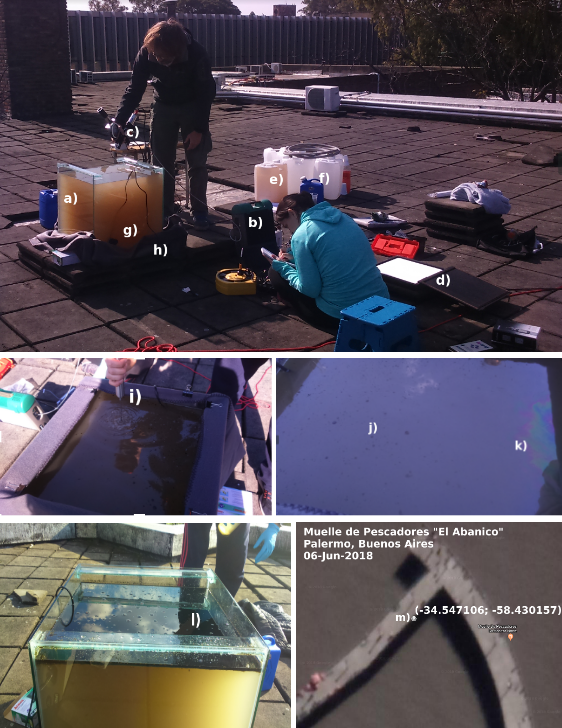
\includegraphics[width=0.75\textwidth]{oil/figures/fotos}
    \caption[Fotografías de dispositivos utilizados y fenómenos observados durante el experimento de detección de hidrocarburos.]{Fotografías de dispositivos utilizados y fenómenos observados durante el experimento. a) Pecera de vidrio de $50 \times 50 \times 50 cm^{3}$ y espesor de 6 mm. b) Radiómetro hiperespectral ASD (CONAE). c) Fibra óptica del radiómetro, $FOV = 8\degree$ (CONAE). d) Placa cuasi lambertiana Spectralon (CONAE). e) Bidones plásticos conteniendo la muestra de 125 litros de agua sustraída del RdP (m). f) Bidón plástico reforzado conteniendo la muestra 1 litro de aceite para motor. g) Motor mezclador, utilizado para la resuspensión de sedimentos (adherido a una cara lateral interna de la pecera). h) Manta opaca utilizada para evitar la intromisión de luz natural por las caras laterales de la pecera. i) Espumador, utilizado como agente emulsionante de la mezcla agua-aceite. j) Régimen de espesor de aceite tipo \textit{Color Natural Discontinuo} (correspondiente al código 4 en la escala de Bonn, ver Cuadro \ref{oil:tab:bonn}, \cite{bonn2004}). k) Régimen de espesor de aceite tipo \textit{Rainbow} (correspondiente al código 2 en la escala de Bonn). l) Vista lateral de la mezcla aceite-agua turbia en el régimen de color continuo (correspondiente a al código 5 en la escala de Bonn). m) Imagen extraída de GoogleMaps del punto de extracción de la muestra utilizada para el experimento.}
    \label{oil:fotos}
    \end{figure}
    
    Para el análisis de los datos obtenidos, se compararon los datos radiométricos (ASD) y turbidimétricos (HACH) obtenidos \textit{in situ} provenientes de diversas campañas de mediciones realizadas en el RdP en el período 2012-2017 (cf. \S \ref{dat}) con los datos experimentales medidos \textit{ad hoc}. A su vez, se utilizaron reflectancias del agua obtenidas por el sensor OLCI-A a bordo del satélite Sentinel-3A de la ESA. Las mismas provienen del conjunto de imágenes detallado en el Cuadro \ref{oil:tab:olci}.


    \begin{table}
        \caption{Subregiones de imágenes de S3-A/OLCI utilizadas en el presente capítulo.}
        \begin{tabular}{|l|l|l|}
        \hline
        \textbf{Región}          & \textbf{Hora de adquisición} & \textbf{Líneas/Píxeles} \\ \hline
        \textbf{RdP} & 2016-08-17T12:55:02Z          & 1347-1636; 1258-1528    \\ \hline
        \textbf{RdP} & 2016-11-10T12:51:59Z          & 1057-1446; 521-685      \\ \hline
        \textbf{RdP} & 2016-11-29T12:58:49Z          & 1643-1796; 1218-1332    \\ \hline
        \textbf{RdP} & 2017-01-14T13:06:26Z          & 2254-2589; 838-1052     \\ \hline
        \textbf{Bahía Blanca}    & 2016-10-09T13:22:33Z          & 2359-2701; 970-1094     \\ \hline
        \end{tabular}
        \label{oil:tab:olci}
    \end{table}

    Para evitar la decantación de los sedimentos suspendidos en el agua, se colocó un motor de circulación en el fondo de la pecera que forzó movimientos de mezcla del fluido durante el experimento. Para minimizar el impacto sobre la rugosidad superficial que generaban dichos movimientos, y que eventualmente habrían impactado en las mediciones radiométricas, el mismo fue apagado durante las mediciones. El viento y el oleaje, los típicos forzantes de las superficies de los cuerpos de agua terrestres suelen emulsionar la mezcla entre los hidrocarburos derramados y el agua (Leifer et al. 2012 \cite{leifer2012}, Clark et al. 2010 \cite{clark2010}); por lo cual fue necesario intentar imitar dicho estado de emulsión. Para lograr esto, se utilizó un agitador o espumador doméstico.
    El radiómetro utilizado para obtener las reflectancias del agua fue el ASD de la CONAE siguiendo el protocolo descrito en detalle en la \S \ref{dat:s:asd}, donde se asumió un coeficiente de Fresnel de $0.0256$, siguiendo lo explicitado por Mobley 1999 \cite{mobley1999} para viento en calma; es decir, superficie planar (aproximación adecuada para la interfase agua-aceite-aire de nuestra muestra). Previo al vertido del hidrocarburo, se tomó una muestra del agua dentro de la pecera y se recalculó la turbidez de la misma, resultando de $(143.5\pm0.5) FNU$. Estimamos que esta leve disminución de la turbidez se debe al hecho de que la pecera fue previamente enjuagada con agua de red, generando trazas de agua cristalina que luego se mezclaron con la muestra de agua del RdP.
    Debido a que los hidrocarburos presentan densidades menores a las del agua líquida, el mismo se fue posicionando sobre el agua tras su vertido, que formó una interfase emulsionada de agua, aire e hidrocarburo tras la emulsificación generada por el batidor doméstico. A lo largo del vertido se fueron consiguiendo apariencias consistentes con las descritas en el Código del Acuerdo de Bonn, \cite{bonn2004}, detalladas en el Cuadro \ref{oil:tab:bonn}.
    
    \begin{table}
    \caption[Código definido en el Acuerdo de Bonn de 2004, decribiendo la apariencia del hidrocarburo sobre el agua según espesor.]{Código definido en el Acuerdo de Bonn de 2004, decribiendo la apariencia del hidrocarburo sobre el agua según espesor, \cite{bonn2004}.}
    \small
    \begin{tabular}{|l|l|l|l|}
    \hline
    \textbf{Código} & \textbf{Descripción/Apariencia}                                                & \textbf{Espesor [$\mu m$]} & \textbf{Volumen [$l/km^{2}$]} \\ \hline
    \textbf{1}      & Brillo plateado/grisáceo                                                       & 0.04 a 0.30                & 40 a 300                      \\ \hline
    \textbf{2}      & Arcoíris                                                                       & 0.30 a 5.00                & 300 a 5000                    \\ \hline
    \textbf{3}      & Metálico                                                                       &  5.0 a 50                  & 5000 a 50000                  \\ \hline
    \textbf{4}      & \begin{tabular}[c]{@{}l@{}}Color del hidrocarburo\\ (discontinuo)\end{tabular} & 50 a 200                   & 50000 a 200000                \\ \hline
    \textbf{5}      & \begin{tabular}[c]{@{}l@{}}Color del hidrocarburo\\ (continuo)\end{tabular}    & >200                       & >200000                       \\\hline
    \end{tabular}
    \label{oil:tab:bonn}
    \end{table}
    
    El experimento realizado para el presente capítulo es novedoso por dos motivos esenciales: por empezar, es el primer caso en que se intenta medir la reflectancia del agua en un estanque de laboratorio, pero en condiciones de iluminación natural. Por ejemplo, en el trabajo realizado por Bale et al. 1999, \cite{bale1994}, se caracterizó la reflectancia de aguas ópticamente complejas en condiciones controladas de laboratorio bajo la presencia de distintos tipos y concentraciones de sedimentos, pero la experiencia se realizó con una fuente de iluminación artificial.
    Por otro lado, es el primer estudio que intenta caracterizar experimentalmente el impacto sobre la región espectral VIS/NIR/SWIR de derrames de petróleo sobre aguas ópticamente complejas. Estudios previos han encarado la posibilidad de generar algoritmos de detección/caracterización de derrames en el óptico en aguas ópticamente claras (ver revisión detallada en Leifer et al. 2012 \cite{leifer2012}). Por ejemplo, Clark et al. 2010, \cite{clark2010}, observan una señal fuertemente roja bajo la presencia de hidrocarburos en el agua, provenientes del derrame de Deepwater Horizon en el Golfo de México en 2010. Nuestra hipótesis inicial es que la presencia de altas concentraciones de sedimentos en el agua (como es el caso del RdP) impactará fuertemente en la señal medida, así como el tipo de hidrocarburo vertido.
    
    % \subsection{Resumen: Materiales experimentales}
    %     A continuación se enumeran los elementos utilizados para el experimento:
    %     \begin{itemize}
    %         \item Pecera de vidrio de $50\times50\times50 cm^{3}$, 6 mm de espesor.
    %         \item Manta opaca para cobertura lateral.
    %         \item 6 bidones plásticos de 20 litros, 1 de 10 litros, 1 de 5 litros.
    %         \item Balde y cabo para toma de muestra de agua ($\sim125 litros$).
    %         \item 1 bidón reforzado de 5 litros con muestra de 1 litro de aceite de motor.
    %         \item Motor de circulación.
    %         \item Espumador para café.
    %         \item Medidor doméstico de capacidad (para medir contenido vertido de aceite).
    %         \item Radiómetro hiperespectral ASD UV/VIS/NIR/SWIR (CONAE)
    %         \item Fibra óptica + óptica FOV=8$\deg$.
    %         \item Placa cuasi lambertiana Spectralon
    %         \item Laptop y PC para procesamiento.
    %         \item Turbidímetro portátil HACH 2100is.
    % \end{itemize}

\section{Resultados}
\label{oil:s:resultados}

    \subsection{Efecto de la cobertura óptica de los laterales del recipiente}
    \label{oil:s:cobertura}
    
        Como testeo preliminar, se evaluó la influencia de la cobertura lateral de la pecera con una tela negra en las mediciones radiométricas. Para ello se compararon las reflectancias espectrales obtenidas para las estaciones en que no se vertió aceite (ST-01, 02 y 03), de las cuales ST-01 y ST-03 fueron tomadas con cobertura lateral y ST-02 sin cobertura. Los resultados (Figura \ref{oil:reflectancias}) muestran un incremento sustancial de la reflectancia del agua cuando los laterales se encontraban descubiertos en el rango espectral dominado por la dispersión (es decir aprox. 500-800 nm). En los rangos espectrales fuertemente dominados por la absorción (en 400-500 nm: debida a las partículas en suspensión; en 800-1300 nm: debida a las moléculas de agua, cf. Figura \ref{dat:HyperTriOS}), no se observaron cambios sustanciales en la reflectancia. Esto es consistente con lo esperado; debido a que, para que la influencia del borde tenga un efecto apreciable sobre la reflectancia del agua en la región central del estanque, es necesario que la radiación sobreviva al camino óptico comprendido entre el lateral y el centro de la pecera ($\sim 25 cm$). En presencia de una fuerte absorción (cf. Figura \ref{dat:HyperTriOS}), dicha radiación incremental no llegaría al sensor; mientras que en la región espectral dispersiva sí llegaría a atravesar el camino óptico. Si bien finalmente se utilizó la cobertura lateral opaca, los resultados obtenidos en la Figura \ref{oil:borde} indicarían que para obviar el efecto de borde en futuras experiencias de laboratorio, será necesario: o bien aumentar la extensión horizontal del estanque utilizado; o bien considerar turbideces más altas; o bien utilizar bordes espejados de forma tal de minimizar el impacto del efecto de borde sobre las mediciones radiométricas.

        \begin{figure}
            \centering
            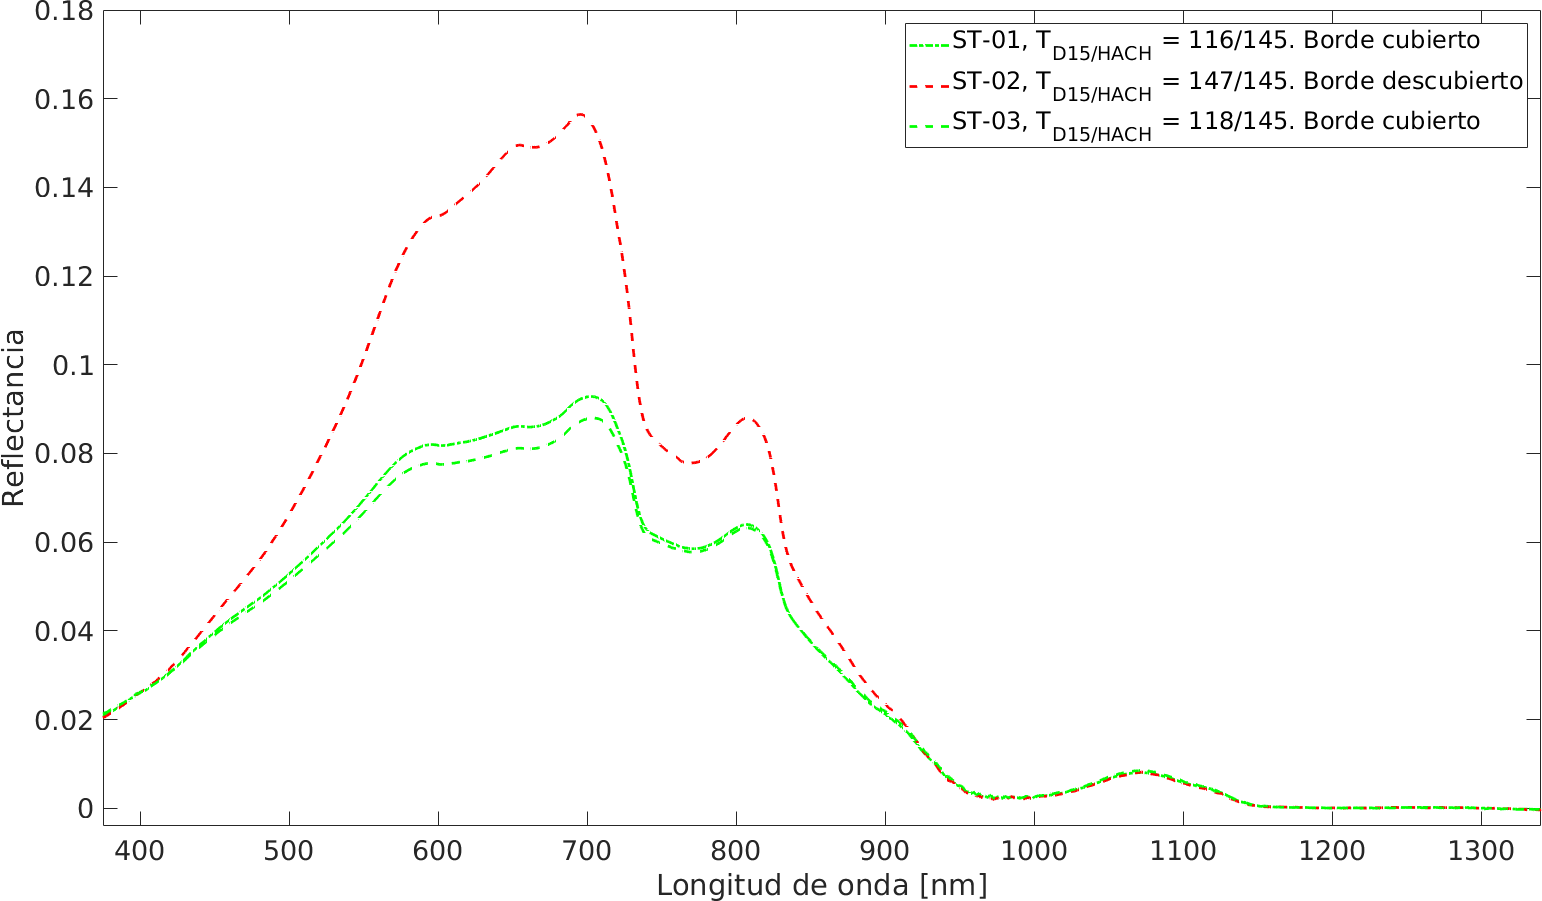
\includegraphics[width=\textwidth]{oil/figures/borde}
            \caption[Firmas obtenidas para las estaciones sin contenido de hidrocarburos.]{Firmas obtenidas para las estaciones ST-01, 02 y 03, es decir, sin contenido de hidrocarburos. Se observan valores apreciablemente más altos para el caso descubierto en la región espectral de $500-800$ nm, dominada por la dispersión de partículas suspendidas; mientras que para las regiones dominadas por la absorción, en torno a 400 nm y por encima de 800 nm, la discrepancia es casi nula.}
            \label{oil:borde}
        \end{figure}

    \subsection{Comparación con reflectancias espectrales de campo}
    \label{oil:s:campo}
        La Figura \ref{oil:reflectancias} muestra las reflectancias del agua obtenidas (en escala jet de colores, representando el espesor de la capa superficial de hidrocarburos), superpuestas a 105 reflectancias medidas sobre el RdP durante diversas campañas realizadas en el período 2013-2017 (en escala de grises, representando el valor de turbidez medido para cada estación, véase \S \ref{dat:s:resultados}). Para las estaciones con menor contenido de hidrocarburos se observan firmas espectrales más comparables con las de campo; pero a medida que el espesor de la capa de hidrocarburos aumenta, la reflectancia tiende a decrecer a lo largo de todo el espectro, a excepción del rango violeta/azul donde se observa un leve incremento para las estaciones correspondientes a los espesores mayores. Dicho fenómeno puede deberse a tres motivos: i)  la inhibición de la absorción debida a las partículas o a sustancias disueltas como el CDOM (cf. \S \ref{qssa:s:iops_spm} y \S \ref{qssa:s:abs_cdom}), dado que la luz interactuaba principalmente con la capa superficial de aceite, el fenómeno de fluorescencia de ciertps hidrocarburos en torno al azul inducida desde el UV (Chen et al. 2017 \cite{chen2017}), o bien la subestimación de la reflexión especular de la radiancia descendente en ángulo recíproco ($L_{sky}$), siendo esto último un problema usual en la metodología de corrección de \textit{skyglint} (ver Ec. \ref{dat:eq:rhoWField}).
        
        \begin{figure}
            \centering
            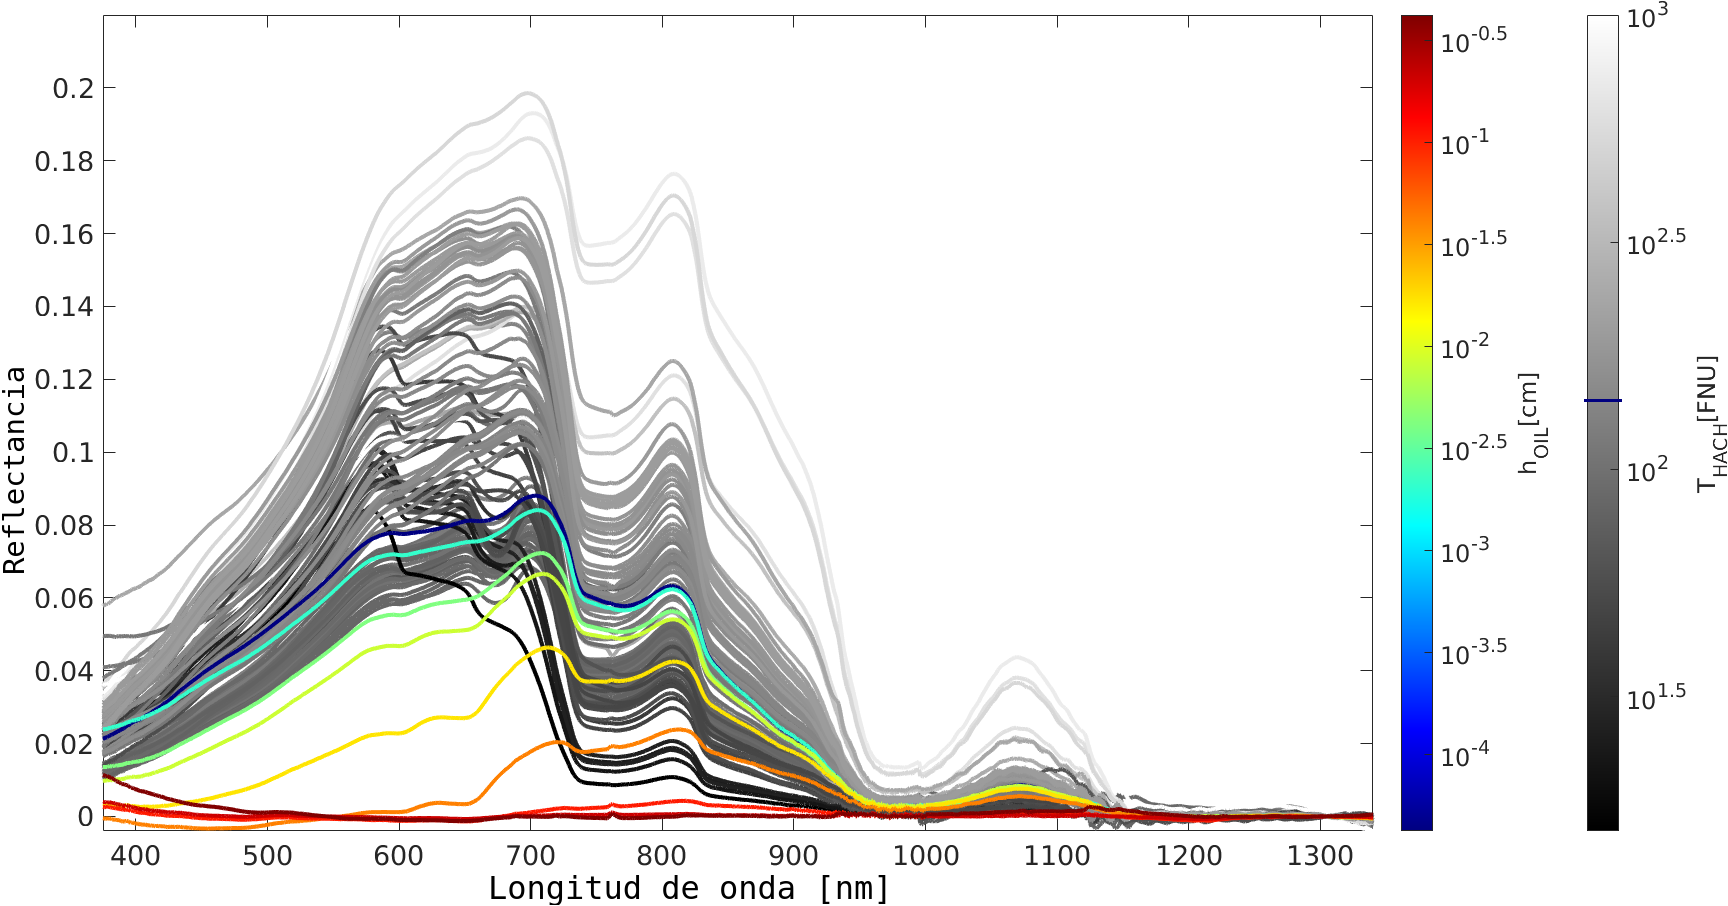
\includegraphics[width=\textwidth]{oil/figures/reflectancias}
            \caption[Reflectancias del agua tomadas en campañas del RdP y sobre la muestra con hidrocarburos.]{Reflectancias del agua tomadas en campañas de mediciones de campo en el RdP (en escala de grises representando la turbidez medida), superpuestas a las reflectancias de las estaciones ST-03 a 11 medidas sobre la pecera (en escala de colores jet representando el espesor equivalente del hidrocarburo utilizado). Sobre la escala de turbideces está marcado el valor medido para ST-03 (espesor nulo), de $(143.5\pm0.5) FNU$.}
            \label{oil:reflectancias}
        \end{figure}
    
        En general, a primera vista, parecería que el efecto que produce la adición de hidrocarburos sobre la muestra es el oscurecimiento general de la misma, por lo que \textit{a priori} podría establecerse una equivalencia entre agregar hidrocarburo y quitar sedimento a la muestra. Sin embargo, se observa que las características espectrales de las firmas de aguas complejas en presencia de hidrocarburos es marcadamente distinguible de las tomadas en el campo.
        Una forma de evaluar esto es analizando la relación entre las reflectancias del agua en 865 nm (NIR) y 620 nm (rojo). Tal como fue expuesto en \S \ref{dat:s:dog15} y \S \ref{dat:s:spmNech10}, en trabajos anteriores, se propuso una relación tipo \textit{Michaelis-Menten}, \cite{michaelis2011}, entre las reflectancias en la región del rojo e infrarrojo cercano y otros parámetros biogeofísicos o bioópticos, como el SPM (Ec. \ref{dat:eq:nechad2010}) o la turbidez (Ec. \ref{dat:eq:dogliotti2015}). Es posible inferir a su vez una relación de tipo Michaelis-Menten entre las reflectancias entre estas bandas, es decir:
    
        \begin{equation}
            \rho_{w}(620) = \frac{\rho_{w}(865)}{(m_{0}^{-1} + S_{\infty}^{-1}\rho_{w}(865))}
            \label{oil:eq:michaelis}
        \end{equation}
    
        \noindent
        donde $m_{0}$ es la pendiente en el régimen lineal, pues $\rho_{w}(620) = m_{0} \times \rho_{w}(865)$ a valores bajos de $\rho_{w}(865)$, y $S_{\infty}$ es la reflectancia de saturación de 620 nm: $\rho_{w}(620) \rightarrow S_{\infty}$ a valores altos de $\rho_{w}(865)$. En la Figura \ref{oil:saturaciones} se observa dicho comportamiento tanto para los datos radiométricos medidos \textit{in situ} como para los píxeles obtenidos de subregiones de imágenes OLCI. Si bien existe una gran variabilidad alrededor del ajuste de Michaleis-Menten, los valores de pendiente en el origen y saturación se mantienen mayor a la unidad y mayor a cero, respectivamente, indicando que la saturación de la reflectancia a 620 nm ocurre a menores valores de SPM que la correspondiente a la banda NIR (865).
        %
        Sin embargo, se observa una relación de Michaelis-Menten inversa para el caso de muestras contaminadas con hidrocarburos a turbidez constante: es decir, la banda de 865 nm \textit{satura} antes que la de 620 nm a valores de espesor de hidrocarburos cada vez más pequeños. Esto se traduce en valores de pendiente en el origen y saturación menor a la unidad y menor a cero, respectivamente. Este resultado indica que la razón de las reflectancias en estas dos bandas podría conformar un índice óptico eficiente a la hora de evaluar la presencia de hidrocarburos en aguas ópticamente complejas.%; dado que evidentemente el comportamiento espectral ante variaciones debidas a los sedimentos es marcadamente distinto al comportamiento que se observó al variar el espesor de la capa de derrame.
        
        \begin{figure}
        \centering
        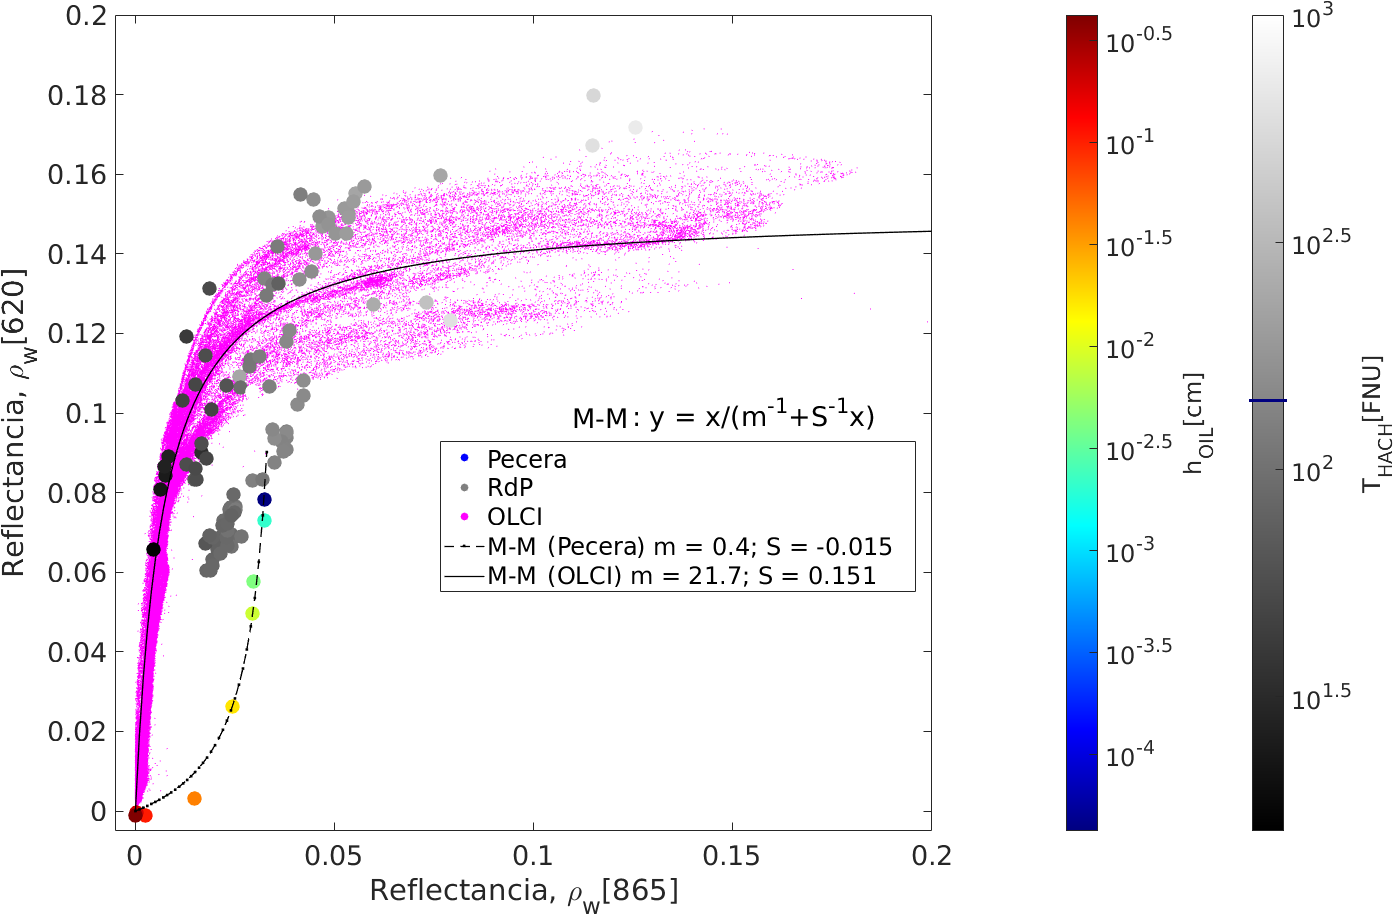
\includegraphics[width=\textwidth]{oil/figures/saturaciones}
        \caption[Reflectancias del agua en 620 nm vs. 865 nm, tomadas en campañas del RdP y sobre la muestra con hidrocarburos.]{Reflectancias del agua en 620 nm vs. 865 nm. En magenta, se grafican los píxeles de las imágenes S3-A/OLCI detalladas en el Cuadro \ref{oil:tab:olci}. En escala de grises (representando la turbidez asociada a cada estación), las mediciones radiométricas adquiridas \textit{in situ} en el RdP. En escala jet de colores (representando el espesor de la capa de hidrocarburos), las mediciones de laboratorio (ST-03 a ST-11, Cuadro \ref{oil:tab:estaciones}). Los ajustes del tipo Michaelis-Menten (Ec. \ref{oil:eq:michaelis}) se grafican en línea punteada y sólida para los datos de la pecera y de OLCI, respectivamente.}
        \label{oil:saturaciones}
        \end{figure}

    \subsection{Otros índices potencialmente útiles para la detección y caracterización de derrames}
    \label{oil:s:indices}
    
        La relación característica entre las reflectancias en 620 nm y 865 nm a turbidez fija - comentada en la sección anterior - es una de las magnitudes ópticas,  entre otras,  que resultaron sensibles a la adición de hidrocarburos a la muestra de agua.
        Una magnitud que a simple vista fue variando en las diferentes estaciones fue la luminosidad total (Figura \ref{oil:luminosidad}). La misma fue calculada a partir de la composición RGB de las reflectancias utilizando la función \textit{color.rgb2lab} del módulo \textit{skimage} de Python (íd. \S \ref{cam:s:identificacion}); y esta a su vez habiendo computado el triplete 620 nm (R), 560 nm (G) y 442 nm (B) a cada reflectancia medida, utilizando las respuestas espectrales de OLCI asociadas a dichas bandas (muy similares a las de MERIS, MODIS o SABIA-Mar). Se observa un marcado descenso de la luminosidad a medida que aumenta el espesor de hidrocarburos, indicando que también podría ser una magnitud óptica sensible a la presencia de hidrocarburos en aguas ópticamente complejas.

        \begin{figure}
        \centering
        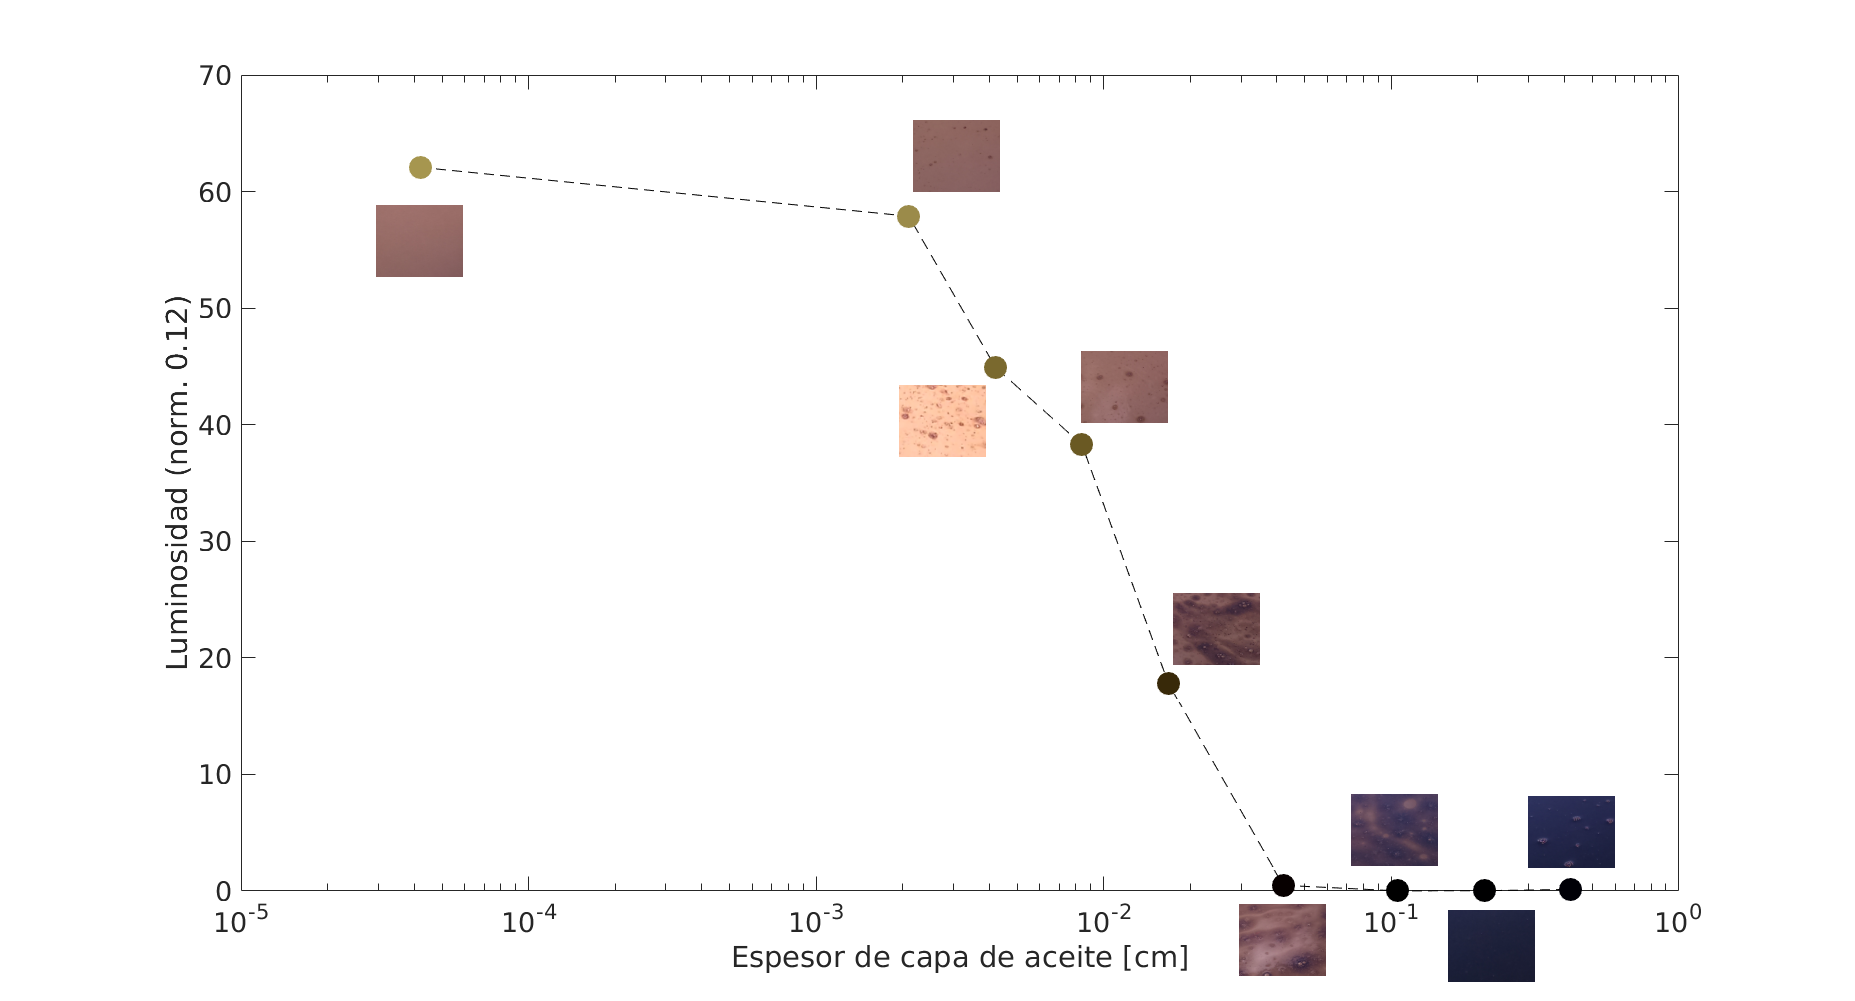
\includegraphics[width=\textwidth]{oil/figures/luminosidad}
        \caption[Luminosidad en función del espesor de la capa de aceite.]{Luminosidad [0-100] correspondiente al espacio CIE La$^{*}$b$^{*}$ 1976, \cite{cie2016}, calculada a partir de la reflectancia medida, en función del espesor de la capa de aceite (en cm). Al costado de cada punto graficado, las fotografías tomadas durante cada respectiva estación.}
        \label{oil:luminosidad}
        \end{figure}
    
        Otras dos magnitudes ópticas resultaron fuertemente sensibles a la presencia de hidrocarburos (por encima de los $20 \mu m$ de espesor): La turbidez, estimada a partir del algoritmo de Dogliotti et al. 2015 (Ec. \ref{dat:eq:dogliotti2015}) aplicado sobre las reflectancias medidas, resultó fuertemente decreciente con la variación de espesor en el rango $[20-120] \mu m$; y la razón violeta(400 nm)/rojo(620 nm) resultó fuertemente creciente en el rango $[120-4000] \mu m$. Ambas magnitudes podrían combinarse para optimizar la sensibilidad de un producto que compute el espesor de la capa de hidrocarburos en aguas ópticamente complejas.
    
        \begin{figure}
            \centering
            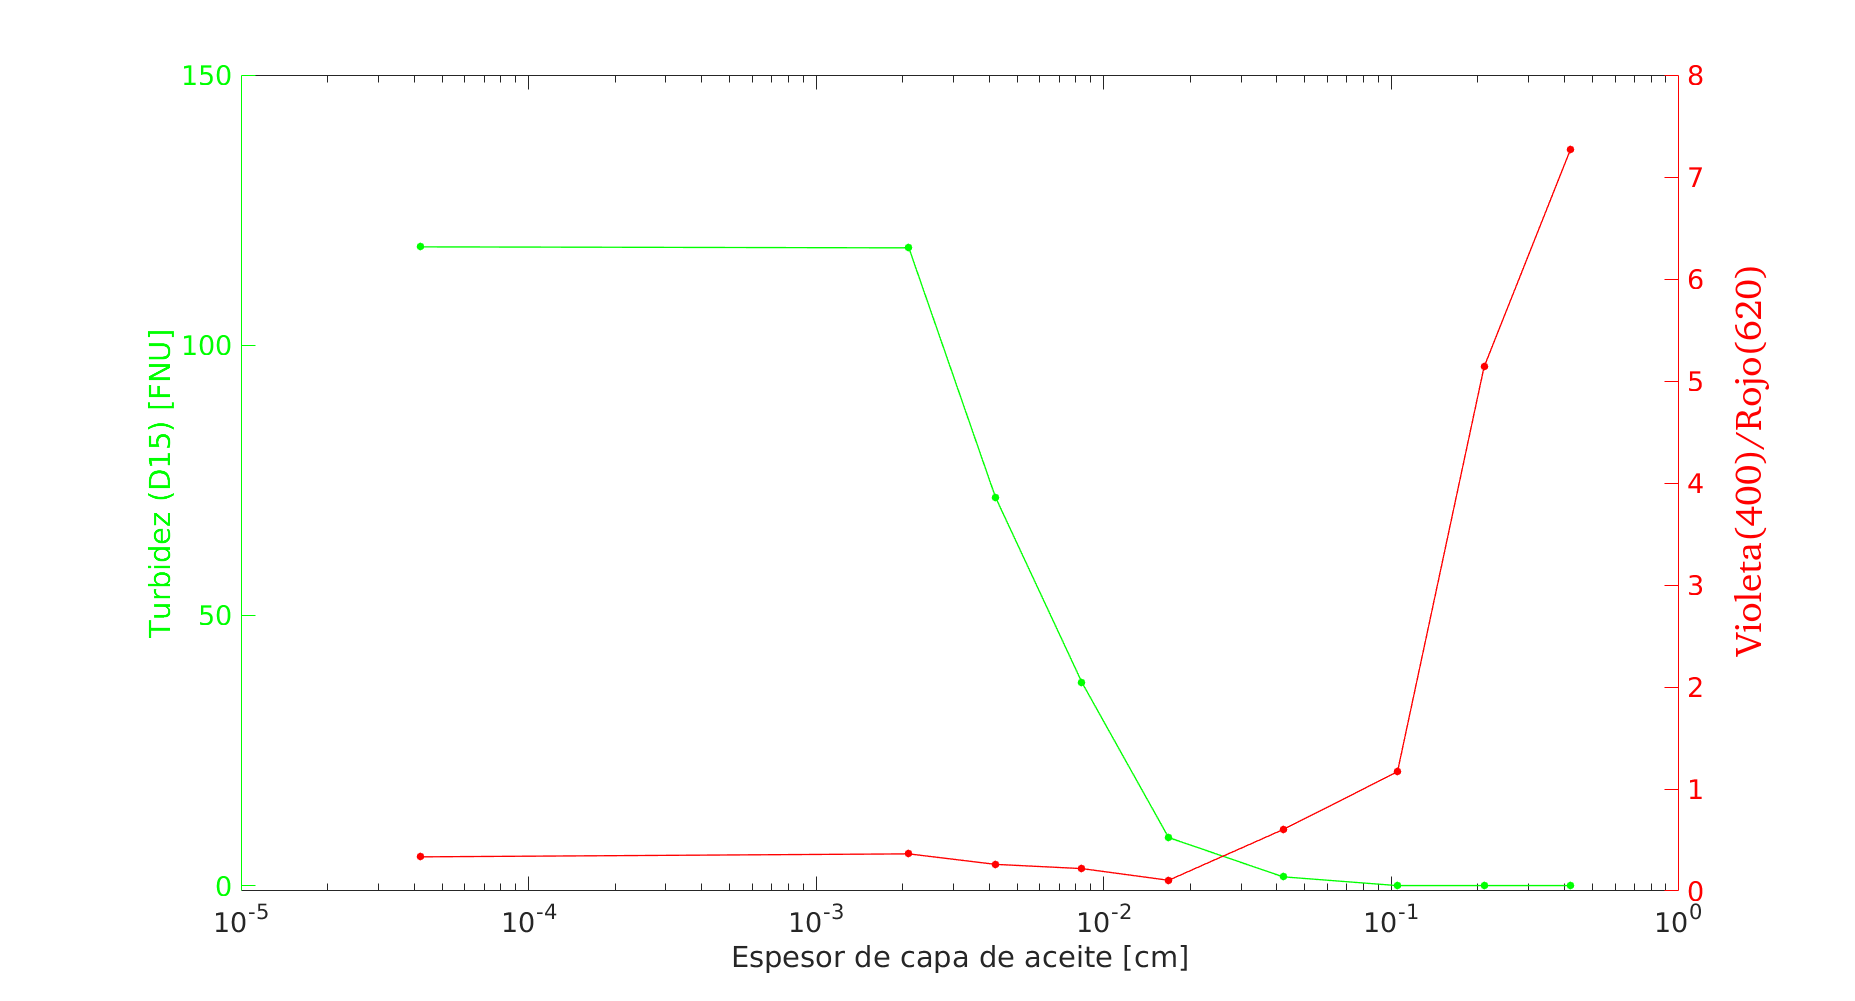
\includegraphics[width=\textwidth]{oil/figures/otrosIndices}
            \caption[Turbidez y razón violeta(400)/rojo(620) en función del espesor de la capa de aceite.]{Turbidez estimada a partir del algoritmo de Dogliotti et al. 2015 (Ec. \ref{dat:eq:dogliotti2015}), aplicado sobre las reflectancias medidas, y razón violeta(400)/rojo(620) en función del espesor de la capa de aceite (en cm).}
            \label{oil:otrosIndices}
        \end{figure}

    \section{Conclusiones}
    \label{oil:s:conclusiones}
        El objetivo de este capítulo fue explorar la potencial complementariedad del sensoramiento remoto en la región óptica del espectro para la caracterización de derrames hidrocarburíferos en aguas ópticamente complejas, como las del RdP.
        %
        Para ello, se consiguió reproducir una muestra de aguas turbias emulsionada con diferentes espesores de hidrocarburos a escala de laboratorio y bajo condiciones de iluminación natural, sobre la cual se realizaron mediciones radiométricas. A partir de los resultados de dichas mediciones, se establecieron potenciales índices espectrales que permitirían discriminar la presencia de hidrocarburos de la varibilidad natural asociada a diferentes valores de SPM. Entre estos índices se hallan el cociente de reflectancias roja/infrarroja, así como la luminosidad, la turbidez o el cociente violeta(400 nm)/rojo(620 nm).
        %
        Así como afirman Brekke et al. 2005, \cite{brekke2005}, sostenemos que, a pesar de que los instrumentos SAR tienen la ventaja de que pueden adquirir imágenes de los océanos y las zonas costeras día y noche independientemente de las condiciones meteorológicas (no válido para los sensores ópticos), la intensidad del viento influye en el nivel de retrodispersión y la visibilidad de las manchas en la superficie del mar, haciendo que las manchas de petróleo sean visibles por sensores SAR sólo para un rango limitado de velocidades del viento. Asimismo, las imágenes SAR serán siempre más escasas por limitaciones de potencia de un sensor activo. Esto implica que puede ser altamente favorable contar con algoritmos complementarios basados en la información que proveen los sensores de la región reflectante del espectro (como OLCI o SABIA-Mar) para combinarla con la información provista por los sensores de tecnología SAR como es el caso de la misión SAOCOM.
        Es necesario ampliar los casos de estudio contemplados, agregando otros tipos de hidrocarburos y variando las concentraciones de sedimentos presentes en el agua ópticamente compleja. A su vez, es necesario continuar caracterizando el impacto del borde del estanque a diferentes condiciones, como pueden ser la ampliación horizontal del mismo, el estudio de muestras con valores de turbidez mayores o la posibilidad de considerar bordes espejados de forma tal de emular una extensión horizontal mayor de la muestra considerada.
